\documentclass[a4paper,openright,12pt]{report}
\usepackage[spanish]{babel} 
\usepackage[latin1]{inputenc} 
\usepackage{graphicx}

\graphicspath{{images/pdf/}}
\usepackage{cite} % para contraer referencias
\usepackage{url} 
\begin{document}
\chapter{Marco Conceptual}
Este capitulo pretende definir todos los conceptos vinculados con el desarrollo del proyecto, en los aspectos de gobernanza en SOA, versionados y calidad de servicios.
\section{Gobernanza en SOA}
\section{Versionado de Servicios}
\section{Calidad de Servicios}
La calidad de los servicios es un elemento importante que permite determinar la facilidad de uso, utilidad y rendimiento del servicio entre otros factores.
\subsection{Metamodelo de calidad}
Un metamodelo de calidad permite definir distintos niveles para evaluar la calidad de un servicio. El metamodelo basico es "Quality Abstract" que contiene la siguiente estructura.
\begin{figure} [h]
\centering
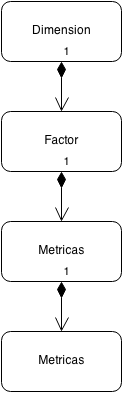
\includegraphics[width=0.5cm]{images/pdf/metamodelo_de_calidad.png}
	\caption{Niveles del Metamodelo de Calidad Absrtacto}
  	\label{figura:metamodelo_de_calidad}
\end{figure}

La figura \ref{figura:metamodelo_de_calidad} nos indican los siguientes niveles.

			\begin{enumerate}
				\item Dimension: Es el aspecto de la calidad correspondiente a la perspectiva que brinda el mayor nivel de abstraccion de la misma.\cite{seminario_CSI_2008}
				\item Factor: Se ubica en el nivel inmediato inferior a la dimension por lo que corresponde a un aspecto particular de la dimension de la calidad. Un factor pude ser mas adecuado que otro para algun tipo de porblema o aplicacion que se este analizando.
				\item Metrica: La metrica corresponde a un instrumento que define una forma de medir un factor de calidad. Puede haber diferentes metricas para el mismo factor, las cuales miden el factor desde diferentes puntos de vista. Consta de tres elementos que tienen que estar bien definidos
				\begin{enumerate}
				\item Semantica (define como se mide la metrica, le da significado)
				\item Unidad de medida (es la cantidad en terminos de magnitud o porcentaje)
				\item Granularidad de la medida (especificidad a la que se define un nivel de detalle)
				\end{enumerate}
				\item Metodo: El metodo corresponde al proceso por el cual se implementa la metrica. Puede haber mas de un metodo que implemente la misma metrica. La implementacion del metodo depende del dominio de la aplicacion en concreto y de aspectos de bajo nivel como pueden ser la estructura de datos que es objeto de estudio.
			\end{enumerate}

\bibliographystyle{acm}
\bibliography{biblio}
\end{document}
